\documentclass{article}
\usepackage{graphicx}
\usepackage{float}
\usepackage{amsmath}

\title{Labwork 4: Threads}
\author{Vu Ha Vy -- 2540112}
\date{\today}

\begin{document}

\maketitle

\section{2D CUDA Implementation}
In Labwork 3, the image was flattened into a 1D array, but in Labwork 4, threads are used in a 2D grid that maps directly to image coordinates $(x, y) = (\text{width}, \text{height})$.  The remaining pipeline is the same as in Labwork 3, where the image is transferred to device memory, processed by the kernel, and then copied back to host memory. \\

\noindent\textit{@cuda.jit} \\
\textit{def grayscale(src, dst):} \\
\textit{\hspace*{1.5em}tidx = cuda.threadIdx.x + cuda.blockIdx.x * cuda.blockDim.x} \\
\textit{\hspace*{1.5em}tidy = cuda.threadIdx.y + cuda.blockIdx.y * cuda.blockDim.y} \\
\textit{\hspace*{1.5em}g = np.uint8((src[tidy, tidx, 0] + src[tidy, tidx, 1] + src[tidy, tidx, 2]) / 3)} \\
\textit{\hspace*{1.5em}dst[tidy, tidx, 0] = dst[tidy, tidx, 1] = dst[tidy, tidx, 2] = g} 

\section{Qualitative Results}

\begin{figure}[H]
\centering
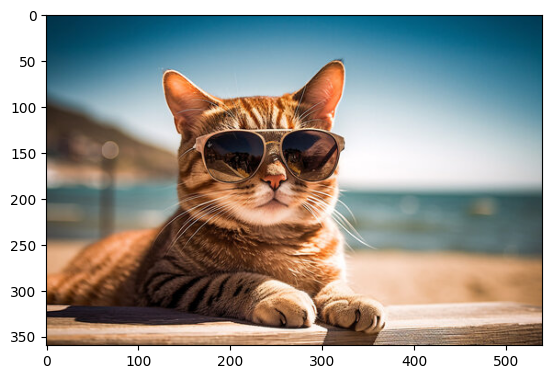
\includegraphics[width=0.73\textwidth]{images/input.png}
\caption{Original input image.}
\end{figure}

\subsection*{Fixed Grid Size}
This experiment uses a fixed grid size of $\text{gridSize} = (8, 8)$ with $\text{blockSize} = (32, 32)$, as in the lecture slide. \\

The total number of threads is $8 \times 32 = 256$ in width and $8 \times 32 = 256$ in height. If the image dimensions exceed $256 \times 256$, we can see that only a portion of the image is processed.

\subsection*{Dynamic Grid Size}
To ensure full coverage of the image, the grid dimensions are computed based on the image's height and width: \\

\noindent\textit{blockSize = (32, 32)} \\
\textit{gridSize = (math.ceil(width / blockSize[0]), math.ceil(height / blockSize[1]))} \\
\textit{grayscale[gridSize, blockSize](devSrc, devDst)}

\begin{figure}[H]
\centering
\begin{minipage}{0.47\textwidth}
  \centering
  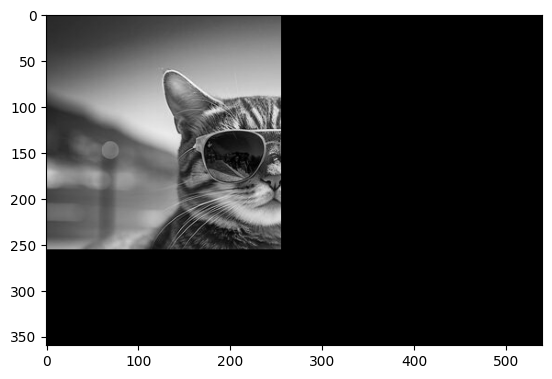
\includegraphics[width=\textwidth]{images/fixed.png}
  \caption{Fixed grid size output.}
\end{minipage}
\hfill
\begin{minipage}{0.47\textwidth}
  \centering
  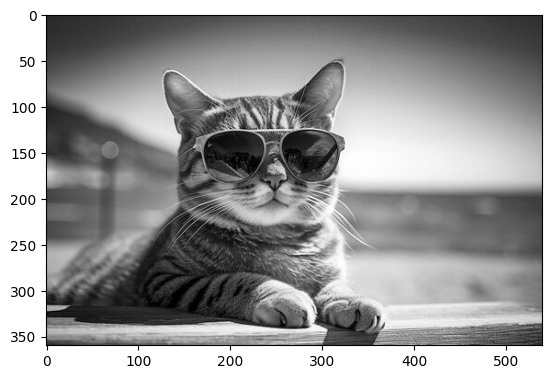
\includegraphics[width=\textwidth]{images/dynamic.png}
  \caption{Dynamic grid size output.}
\end{minipage}
\end{figure}

\section{Quantitative Results}

Experiments were tested across different 2D block configurations and compared against the 1D kernel execution times from Labwork 3.

\begin{table}[H]
\centering
\renewcommand{\arraystretch}{1.5}
\begin{tabular}{|c|c|c|c|c|}
\hline
\textbf{Threads/ 1D Block} & \textbf{2D Block} & \textbf{Grid Size} & \textbf{1D Time (s)} & \textbf{2D Time (s)} \\ \hline
64 & $(8, 8)$ & $(68, 45)$ & 0.001091 & 0.001621 \\ \hline
128 & $(8, 16)$ & $(68, 23)$ & 0.003341 & 0.001333 \\ \hline
256 & $(16, 16)$ & $(34, 23)$ & 0.001880 & 0.000939 \\ \hline
512 & $(16, 32)$ & $(34, 12)$ & 0.001700 & 0.000998 \\ \hline
\end{tabular}
\caption{Running Time Comparison Between 1D and 2D CUDA Kernels}
\end{table}

\begin{figure}[H]
\centering
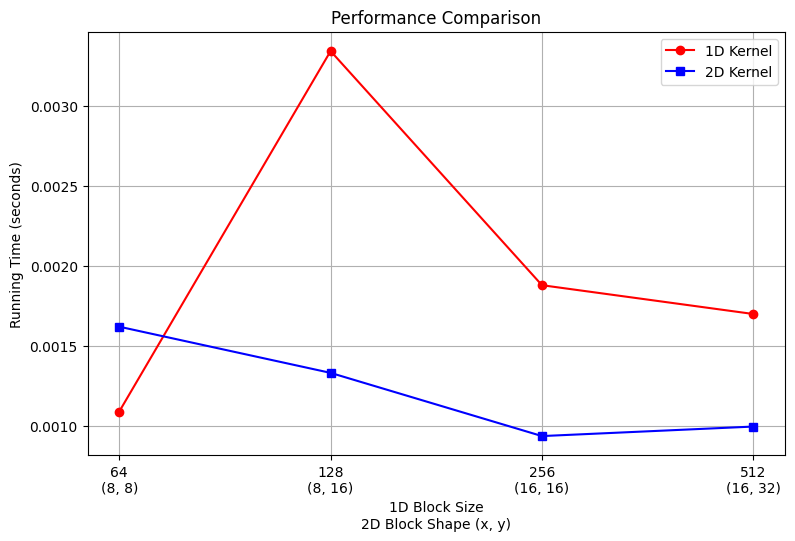
\includegraphics[width=1\textwidth]{images/compare.png}
\caption{Running Time Comparison Between 1D and 2D CUDA Kernels}
\end{figure}

In the 2D implementation, when the block size increase from $(8, 8)$ with 64 threads to $(16, 16)$ with 256 threads, processing time drops from $0.001621\,\text{s}$ down to a minimum of $0.000939\,\text{s}$. This improvement occurs because larger blocks use the hardware resources of the GPU more effectively. However, increasing the size further to $(16, 32)$ causes execution time to rise slightly to $0.000998\,\text{s}$, indicating that $(16, 16)$ provides the optimal balance between thread count and resource limits per block. \\

When comparing the two implementations, the 2D kernel generally outperforms the 1D version across most block configurations. Except for the smallest size of 64 threads where the 1D kernel is faster ($0.001091\,\text{s}$ vs $0.001621\,\text{s}$). The 2D kernel achieves speedups $1.70\text{x}$ to $2.51\text{x}$ for larger configurations. Mapping threads directly in two dimensions allows the GPU to access image pixel data much more efficiently in memory compared to the flattened 1D approach.

\pagebreak
\section{Exercises}

\subsection*{Exercise 1}
\begin{itemize}
    \item $8 \times 8$ (64 threads): The SM has 8 blocks ($8 \times 64 = 512$ threads total), so it only runs at $50\%$ occupancy.
    \item $16 \times 16$ (256 threads): We can use 4 blocks, so that $4 \times 256 = 1024$ threads total, giving full $100\%$ occupancy.
    \item $32 \times 32$ (1024 threads): Limit of the GPU is 512 threads per block.
\end{itemize}
\noindent\textbf{Answer:} $16 \times 16$

\subsection*{Exercise 2}

\begin{itemize}
    \item 128 threads/block: Using 4 blocks, we have $4 \times 128 = 512$ threads total.
    \item 256 threads/block: Using 4 blocks, we have $4 \times 256 = 1024$ threads total.
    \item 512 threads/block: Using 3 blocks, we have $3 \times 512 = 1536$ threads total, reaching maximum thread capacity.
    \item 1024 threads/block: Using 1 block, we have $1 \times 1024 = 1024$ threads total.
\end{itemize}
\noindent\textbf{Answer:} 512 threads/block


\subsection*{Exercise 3}

To process 2000 elements with a block size of 512, we need $\lceil 2000 / 512 \rceil = 4$ blocks. Running 4 blocks gives $4 \times 512 = 2048$ total threads. So 2000 will do the actual work, and the remaining 48 threads will wait. \\

\noindent\textbf{Answer:} 2048 threads

\end{document}